\chapter{\textsl{Seifert-Kampen}定理}

\section{\textsl{Abelian}群的直接和}

设$G$是一个\textsl{Abelian}群,$\{G_\alpha\}_{{\alpha\in J}}$为$G$的子群的一个加标族,如果$G$中的每一个元素$x$可以表示为群族$G_\alpha$中有限个成员之和,则称群族$G_\alpha$\textbf{生成}$G$。

设群族$G_\alpha$生成$G$,则称$G$为群族$G_\alpha$的\textbf{和}。记作
\begin{equation}
    G=\sum_{\alpha\in J}G_\alpha
\end{equation}

设群族$G_\alpha$生成$G$,并且对于每一个$x\in G$,$x$的表示$x=\sum x_\alpha$是唯一的,也就是说,对于每个$x\in G$,只有一个\textsl{J-串}$(x_\alpha)_{\alpha\in J}$使得除有限个$\alpha$外都有$x_\alpha=0$,并且$x=\sum x_\alpha$。这称为群族$G_\alpha$的\textbf{直和},记作
\begin{equation}
    G=\oplus_{\alpha\in J} G_\alpha    
\end{equation}

\subsection*{\textsl{直和的扩展条件}}

\begin{mdframed}
    \begin{lemma}
        设$G$是一个\textsl{Abelian}群,$\{G_\alpha\}$是$G$的子群的一个族,如果$G$为群族$G_\alpha$的直和,则$G$满足以下条件:
        \begin{enumerate}[itemindent=2em]
            \item[$(*)$] 对于任何\textsl{Abelian}群$H$以及任何同态$h_\alpha:G\rightarrow H$的族,存在一个同态$h:G\rightarrow H$,使得对于每一个$\alpha$,$h$在$G_\alpha$上的限制等于$h_\alpha$。
        \end{enumerate}

        此外,$h$还是唯一的,反之,如果群族$G_\alpha$生成$G$并且扩展条件$(*)$成立,则$G$为群族$G_\alpha$的直和。
    \end{lemma}
\end{mdframed}

\begin{mdframed}
    \begin{corollary}
        设$G=G_1\oplus G_2$,假定$G_1$为子群族$\{H_\alpha\}_{\alpha\in J}$的直和,$G_2$为子群族$\{H_\beta\}_{\beta\in K}$的直和,其中指标集$J$与$K$无交,则$G$为子群族$\{H_\gamma\}_{\gamma\in J\cup K}$的直和。
    \end{corollary}
\end{mdframed}

\begin{mdframed}
    \begin{corollary}
        若$G=G_1\oplus G_2$,则$G/G_2$同构于$G_1$。
    \end{corollary}
\end{mdframed}

\subsection*{\textsl{构造群$G$的办法}}

\begin{mdframed}
    \begin{theorem}
        对于给定的\textsl{Abelian}群的一个族$\{G_\alpha\}_{\alpha\in J}$,存在一个\textsl{Abelian}群和单同态的一个族$i_\alpha:G_\alpha\rightarrow G$,使得$G$为群族$i_\alpha(G_\alpha)$的直和。
    \end{theorem}
\end{mdframed}

\subsection*{\textsl{刻画外直和的扩展条件}}

\begin{mdframed}
    \begin{theorem}
        设$\{G_\alpha\}$为\textsl{Abelian}群的一个加标族,$G$是一个\textsl{Abelian}群,$i_\alpha:G_\alpha\rightarrow G$为同态的一个族,如果每一个$i_\alpha$都是单同态,并且$G$是群族$i_\alpha(G_\alpha)$的直和,则$G$满足以下扩展条件:
        \begin{enumerate}[itemindent=2em]
            \item[$(*)$] 对于任何\textsl{Abelian}群$H$以及任何同态族$h_\alpha:G_\alpha\rightarrow H$,存在一个同态$h:G\rightarrow H$,使得对于每一个$\alpha$都有$h\circ i_\alpha=h_\alpha$
        \end{enumerate}

        此外,$h$还是唯一的,反之,如果群族$i_\alpha(G_\alpha)$生成$G$并且扩展条件$(*)$成立,则每一个$i_\alpha$都是单同态,并且$G$为群族$i_\alpha(G_\alpha)$的直和。
    \end{theorem}
\end{mdframed}

\subsection*{\textsl{直和的唯一性定理}}

\begin{mdframed}
    \begin{theorem}
        设$\{G_\alpha\}$为\textsl{Abelian}群的一个族,设$G$和$G'$都是\textsl{Abelian}群,$i_\alpha:G_\alpha\rightarrow G$和$i'_\alpha:G_\alpha\rightarrow G'$,其中$G$是群族$i_\alpha(G_\alpha)$的直和,$G'$是群族$i'_\alpha(G_\alpha)$的直和,
        则存在一个唯一同构$\phi:G\rightarrow G'$,则存在一个唯一同构$\phi:G\rightarrow G'$使得$\phi\circ i_\alpha=i'_\alpha$对于每一个$\alpha$成立。
    \end{theorem}
\end{mdframed}

\subsection*{\textsl{自由Abelian群的扩展条件}}

\begin{define}
    设$G$是一个\textsl{Abelian}群,$\{a_\alpha\}$是$G$中元素的一个加标族,$G_\alpha$是由$a_\alpha$生成的$G$的子群,如果群族$G_\alpha$生成$G$,我们也称元素族$a_\alpha$生成$G$,如果每一个群$G_\alpha$都是无限循环群,并且$G$为群族$G_\alpha$的直和,则称$G$为群族$G_\alpha$的直和,则称$G$为以元素族$\{a_\alpha\}$为\textbf{基}的\textbf{自由Abelian群}。
\end{define}

\begin{mdframed}
    \begin{lemma}[\textbf{\textsl{自由Abelian群的扩展条件}}]
        设$G$是一个\textsl{Abelian}群,$\{a_\alpha\}_{\alpha\in J}$为$G$中元素的一个族,它们生成$G$,则$G$是一个以$\{a_\alpha\}$为基的自由\textsl{Abelian}群的充分必要条件是:对于任何一个\textsl{Abelian群}$H$以及$H$中任意元素的一个族$\{y_\alpha\}$,存在一个$G$到$H$的同态$h$,
        使得$h(a_\alpha)=y_\alpha$对于每一个点$\alpha$成立,这时,$h$是唯一的。
    \end{lemma}
\end{mdframed}

\begin{mdframed}
    \begin{theorem}
        设$G$是以$\{a_1,\cdots,a_n\}$为基的一个自由\textsl{Abelian}群,则$n$是由$G$唯一确定的。
    \end{theorem}
\end{mdframed}

如果$G$具有有限基的自由\textsl{Abelian}群,则$G$的基元素的个数叫做$G$的\textbf{秩}。

\section{群的自由积}

\begin{mdframed}
    \begin{define}
        设$G$是一个群,$\{G_\alpha\}_{\alpha\in J}$为生成$G$的$G$的一个子群族,假设$\alpha\neq \beta$时$G_\alpha\cap G_\beta$仅含有单位元,称$G$为群族$G_\alpha$的\textbf{自由积},
        如果对于任何一个$x\in G$,都唯一地存在含于群组$G_\alpha$并且表示$x$的字,记作
        \begin{equation}
            G=\prod_{\alpha} G_\alpha
        \end{equation}

        对于有限的情形,也记作$G=G_1\times G_2\times\cdots G_n$.
    \end{define}
\end{mdframed}

\subsection*{\textsl{自由积也满足类似于直和的扩展条件}}

\begin{mdframed}
    \begin{lemma}
        设$G$是一个群,$\{G_\alpha\}$为$G$的子群族,若$G$为群族$G_\alpha$的自由积,则$G$满足以下条件
        \begin{enumerate}[itemindent=2em]
            \item[$(*)$] 对于任何群$H$以及任何同态族$h_\alpha:G_\alpha\rightarrow H$,存在一个同态$h:G\rightarrow H$,使得对于每一个$\alpha$,同态$h$在$G_\alpha$上的限制等于$h_\alpha$.
        \end{enumerate}

        此外$h$是唯一的。
    \end{lemma}
\end{mdframed}

\subsection*{\textsl{外自由积}}

\begin{mdframed}
    \begin{define}
        设$\{G_\alpha\}$为群的一个加标族,设$G$是一个群,$i_\alpha:G_\alpha\rightarrow G$为单同态的一个族,使得$G$为群族$i_\alpha(G_\alpha)$的自由积,则称$G$为群族$G_\alpha$相对于单同态族$i_\alpha$的\textbf{外自由积}。
    \end{define}
\end{mdframed}

\subsection*{\textsl{在不同区别同构的群的意义下群$G$是唯一的}}

\begin{mdframed}
    \begin{theorem}
        对于给定的群的一个族$\{G_\alpha\}_{\alpha\in J}$,存在一个群$G$以及单同态的一个族$i_\alpha:G_\alpha\rightarrow G$,使得$G$是群族$i_\alpha(G_\alpha)$的自由积。
    \end{theorem}
\end{mdframed}

\subsection*{\textsl{外自由积的扩展条件}}

\begin{mdframed}
    \begin{theorem}
        设$\{G_\alpha\}$是群的一个族,$G$是一个群,$i_\alpha:G_\alpha\rightarrow G$为同态的一个族,如果每一个$i_\alpha$都是一个单同态,并且$G$为群族$i_\alpha(G_\alpha)$的自由积,则$G$满足以下条件:
        \begin{enumerate}[itemindent=2em]
            \item[$(*)$] 对于任何一个群$H$,以及任何同态的一个族$h_\alpha:G_\alpha\rightarrow H$存在一个同态$h:G\rightarrow H$,使得对于每一个$\alpha$都有$h\circ i_\alpha=h_\alpha$
        \end{enumerate}

        此外$h$是唯一的。
    \end{theorem}
\end{mdframed}

\subsection*{\textsl{自由积的唯一性}}

\begin{mdframed}
    \begin{theorem}
        [\textbf{自由积的唯一性}] 设$\{G_\alpha\}_{\alpha\in J}$是群的一个族,假设$G$和$G'$都是群,$i_\alpha:G_\alpha\rightarrow G$和$i_\alpha':G_\alpha\rightarrow G'$都是单同态族,使得$\{i_\alpha(G_\alpha)\}$和$\{i'_\alpha(G_\alpha)\}$分别生成$G$和$G'$,如果$G$和$G'$分别具有前述引理中的扩展性质,则有一个唯一的同构
        $\phi:G\rightarrow G'$,使得对于每一个$\alpha$有$\phi\circ i_\alpha=i_\alpha'$
    \end{theorem}
\end{mdframed}

\subsection*{\textsl{证明扩展条件决定了自由积}}

\begin{mdframed}
    \begin{lemma}
        设$\{G_\alpha\}_{\alpha\in J}$是群的一个族,假设$G$是一个群,$i_\alpha:G_\alpha\rightarrow G$是同态的一个族,如果扩展条件成立,则对每一个$i_\alpha$都是一个单同态,并且$G$是群族$i_\alpha(G_\alpha)$的自由积。
    \end{lemma}
\end{mdframed}

\begin{mdframed}
    \begin{corollary}
        设$G=G_1\times G_2$,其中$G_1$和$G_2$分别是子群族$\{H_\alpha\}_{\alpha\in J}$和$\{H_\beta\}_{\beta\in K}$的自由积,如果指标集$J$与$K$无交,则$G$为子群族$\{H_\gamma\}_{\gamma\in J\cup K}$的自由积。
    \end{corollary}
\end{mdframed}

这个结论特别蕴含着
\begin{equation}
    G_1\times G_2\times G_3=G_1\times (G_2\times G_3)=(G_1\times G_2)\times G_3
\end{equation}

\subsection*{\textsl{最小正规子群}}

设$x$和$y$都是群$G$中的元素,称$y$\textbf{共轭}于$x$,如果对于每一个$c\in G$,$y=cxc^{-1}$成立,群$G$的正规子群是一个含有群中所有元素的所有元素的所有共轭元的子群。

\begin{mdframed}
    \begin{define}
        设$S$为$G$的一个子集,我们考虑$G$中包含$S$的所有正规子群的交$N$,易见,$N$自身也是$G$的一个正规子群,称为$G$中包含$S$的\textbf{最小的正规子群}。
    \end{define}
\end{mdframed}

\begin{mdframed}
    \begin{theorem}
        设$G=G_1\times G_2$,设$N_i$为$G_i$的正规子群,$i=1,2$,如果$N$是$G$中包含$N_1$和$N_2$的最小正规子群,则
        \begin{equation}
            G/N\cong (G_1/N_1)\times (G_2/N_2)
        \end{equation}
    \end{theorem}
\end{mdframed}

\begin{mdframed}
    \begin{corollary}
        如果$N$是$G_1\times G_2$中包含$G_1$的最小正规子群,则$(G_1\times G_2)/N\cong G_2$
    \end{corollary}
\end{mdframed}


\section{自由群}

\begin{mdframed}
    \begin{define}
        设$\{a_\alpha\}$是$G$中元素的一个族,假设每一个$a_\alpha$生成$G$的一个无限循环子群$G_\alpha$,如果$G$为群$\{G_\alpha\}$
        的自由积,则称$G$为\textbf{自由群},并且称$\{a_\alpha\}$为$G$的一个\textbf{自由生成元组}
    \end{define}
\end{mdframed}

\subsection*{\textsl{自由群由下面的扩展性质刻画}}
\begin{mdframed}
    \begin{lemma}
        设$G$是一个群,$\{a_\alpha\}_{\alpha\in J}$为$G$中元素的一个族,如果$G$是具有自由生成元组$\{a_\alpha\}$的一个自由群,则$G$满足以下条件:
        \begin{enumerate}[itemindent=2em]
            \item[$(*)$] 对于任意给定的群$H$以及任何$H$中的元素的一个族$\{y_\alpha\}$,存在一个同态$h:G\rightarrow H$使得$h(a_\alpha)=y_\alpha$对于每一个$\alpha$成立。
        \end{enumerate}

        此外,$h$是唯一的,反之,如果扩展条件成立,则$G$是具有自由生成元组$\{a_\alpha\}$的自由群。
    \end{lemma}
\end{mdframed}

\subsection*{\textsl{元素族上的自由群}}

设$\{a_\alpha\}_{\alpha\in J}$为任何一个加标族,设$G_\alpha$表示所有形如$a^n_\alpha(b\in \mathbb{Z})$的符号的集合,通过定义
\begin{equation}
    a^n_\alpha\cdot a^m_\alpha=a^{n+m}_\alpha
\end{equation}

使得$G_\alpha$成为一个群,则$a^0_\alpha$为$G_\alpha$的单位元,并且$a^{-n}_\alpha$为$a^n_\alpha$的逆元,将$a^1_\alpha$简记为$a_\alpha$,我们将$\{G_\alpha\}$的外自由积成为\textbf{元素族$a_\alpha$上的自由群}

\subsection*{\textsl{交换子子群}}

如果$G$是一个群,$x,y\in G$,我们用$[x,y]$表示$G$中的元素
\begin{equation}
    [x,y]=xyx^{-1}y^{-1}
\end{equation}

并称其为$x$和$y$的\textbf{交换子},由$G$中所有的交换子生成的子群称为$G$的\textbf{交换子子群}。

\begin{mdframed}
    \begin{theorem}
        对任何$G$,交换子子群$[G,G]$是$G$的一个正规子群,并且商群$G/[G,G]$是一个\textsl{Abelian}群,若$h:G\rightarrow H$为$G$到任何\textsl{Abelian}群$H$的一个同态,则$h$的核包含$[G,G]$,从
        而$h$诱导一个同态$k:G/[G,G]\rightarrow H$。
    \end{theorem}
\end{mdframed}

\begin{mdframed}
    \begin{theorem}
        设$G$是以$a_\alpha$为自由生成元组的自由群,则$G/[G,G]$是一个以$[a_\alpha]$为基的自由\textsl{Abelian}群,这里$[a_\alpha]$表示$G/[G,G]$中$a_\alpha$的陪集。
    \end{theorem}
\end{mdframed}

\subsection*{\textsl{$Betti$数、初等因子,关系子群、有限表示}}

\newpage

\section{\textsl{Seifert-Kampen}定理}

\begin{mdframed}
    \begin{theorem}
        [\textbf{Seifert-van Kampen定理}] 设$X= U \cup V$,其中$U$和$V$是$X$中的开集,假设$U,V$以及$U\cap V$都是道路连通的,$x_0\in U\cap V$。设$H$是一个群,并且
        \begin{equation}
            \phi_1:\pi_1(U,x_0)\rightarrow H,\ \ \phi_2:\pi_1(V,x_0)\rightarrow H
        \end{equation}

        是两个同态,设$i_1,i_2,j_1,j_2$是依照下图所示内射诱导的同态
        \begin{figure}[H]
            \centering
            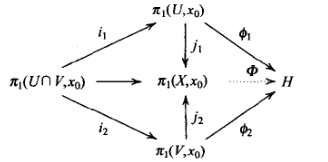
\includegraphics[scale=0.6]{figures/WX20240902-113016@2x.png}
        \end{figure}

        如果$\phi_1\circ i_1=\phi_2\circ i_2$,则存在一个唯一同态$\Phi_1:\pi_1(X,x_0)\rightarrow H$使得$\Phi\circ j_1=\phi_1$和$\Phi\circ j_2=\phi_2$成立
    \end{theorem}
\end{mdframed}

\section{圆周束的基本群}

\section{黏粘$2$维胞腔}

\section{环面和小丑帽的基本群}